% !TeX root = ../dokumentation.tex

\chapter{Sprints}

\section{Sprint 1}
\todo{Beschreibung des Produktincrements}

\section{Ziele Sprint 1}
\todo{Ziel Sprint 1}

\section{Ergebnisse Sprint 1}

\subsection{Produktincrement}
\subsection{Charts}

\subsection{Probleme und Verbesserungen}
\todo{Retro Ergebnisse}


\subsection{Bearbeitete User Storys}

\subsubsection{SKIOS-13 Create Basic Infrastructure}
Das Ticket \enquote{SKIOS-13 Create Basic Infrastructure} hatte folgende User Story:
\begin{quotation}
    Als Product Owner möchte ich die Möglichkeit haben das unser Produkt weltweit sicher erreichbar ist. Um das zu erreichen, muss ein Server mit einer passenden gemietet werden. \\
    \textbf{Acceptance Criteria}
    \begin{itemize}
        \item Die Domain \enquote{Skiosa.de} bestellt und dem Server zugewiesen.
        \item Einen passenden Server bestellt und mit notwendigen Tools wie SSH aufgesetzt.
        \item K3S Basis Installation.
        \item kubectl von Remote erreichbar und eingerichtet.
        \item Firewall Regeln angelegt um nur Web, SSH und Kubectl zuzulassen.
    \end{itemize} 
\end{quotation}
Bearbeitet von Lukas Huida.
Reviewed von Tim Horlacher.

\subsubsection{SKIOS-18 Basic Kubernetes Infra}
Das Ticket \enquote{SKIOS-18 Basic Kubernetes Infra} hatte folgende User Story:
\begin{quotation}
    As a infra member I want a basic Infrastructure based on Kubernetes. This Infrastructure should container some CI/CD pipeline software and examples to implement
    a CI/CD pipeline for our services. \\
    \textbf{Acceptance Criteria}
    \begin{itemize}
        \item Working Ingress-Controller with correct Certs
        \item Self-Hosted Docker-Registry
        \item ArgoCD Setup
        \item Drone.io Setup
        \item SonarQube Setup
        \item Keycloak Setup
        \item HashiCorp Vault Setup (Optional)
    \end{itemize}
\end{quotation}
Bearbeitet von Lukas Huida.
Reviewed von Tim Horlacher.

\subsubsection{SKIOS-9 Create Continous Integration Pipeline}
Das Ticket \enquote{SKIOS-9 Create Continuos Integration Pipeline} hatte folgende User Story:
\begin{quotation}
    As a developer I want my code to be tested and analyzed by sonar after every new commit so that our platform can ensure stability. \\
    \textbf{Acceptance Criteria}
    \begin{itemize}
        \item A pipeline exists for every service.
        \item A commit pipeline is triggered after every commit on a non master branch. This pipeline runs through: unit tests and sonarqube.
        \item A pr pipeline is triggered after a pull requests is created. This pipeline runs through: unit tests, integration tests and sonarqube.
        \item A main pipeline is triggered after a merge of a master branch. This pipeline runs through: unit tests, container build, CD-Script and sonarqube.
    \end{itemize}
\end{quotation}
Bearbeitet von Lukas Huida.
Reviewed von Tim Horlacher.

\subsubsection{SKIOS-10 Create Continous Delivery Pipeline}
Das Ticket \enquote{SKIOS-10 Create Continuos Delivery Pipeline} hatte folgende User Story:
\begin{quotation}
    As a developer I want my code to be delivered to prod after I merge it to master. \\
    \textbf{Acceptance Criteria}
    \begin{itemize}
        \item pipeline is triggered after merge to master
        \item pipeline tests code with unit/sonar before merge (is already managed by ci-pipeline)
        \item pipeline tests code with newman after merge → fail leads to rollback
    \end{itemize}
\end{quotation}
Bearbeitet von Lukas Huida.
Reviewed von Jonas Eppard.

\subsubsection{SKIOS-21 Initialize Keycloak}
Das Ticket \enquote{SKIOS-21 Initialize Keycloak} hatte folgende User Story:
\begin{quotation}
    As a developer I would like to have Keycloak setup so that we can test its usefulness. \\
    \textbf{Acceptance Criteria}
    \begin{itemize}
        \item A Keycloak server is running in our cluster and is reachable.
    \end{itemize}
\end{quotation}
Bearbeitet von Lukas Huida.
Reviewed von Tim Horlacher.

\subsubsection{SKIOS-30 Preliminary Core service}
Das Ticket \enquote{SKIOS-30 Preliminary Core service} hatte folgende User Story:
\begin{quotation}
    As a developer I want to have a basic core service with some boilerplate and mock endpoints to get started in the frontend. \\
    \textbf{Acceptance Criteria}
    \begin{itemize}
        \item be able to fetch mock articles with graphql
    \end{itemize}
\end{quotation}
Bearbeitet von Lukas Huida.
Reviewed von Tim Horlacher.

\subsubsection{SKIOS-37 Decision of Programming Database}
Das Ticket \enquote{SKIOS-37 Decision of Programming Database} hatte folgende User Story:
\begin{quotation}
    As a developer I need to know which database is used, to know which database connector for ORMs are needed. \\
    \textbf{Acceptance Criteria}
    \begin{itemize}
        \item A decision of a database is done
        \item The decision is documented in Confluence
    \end{itemize}
\end{quotation}
Bearbeitet von Lukas Huida.
Reviewed von Jonas Eppard.

\subsubsection{SKIOS-49 Create Example Service}
Das Ticket \enquote{SKIOS-49 Create Example Service} hatte folgende User Story:
\begin{quotation}
    As a developer I want an example service to test the CI/CD pipeline. \\
    \textbf{Acceptance Criteria}
    \begin{itemize}
        \item An example service exists
        \item A example deployment is created
        \item A example CI pipeline is working with the example service
    \end{itemize}
\end{quotation}
Bearbeitet von Lukas Huida.
Reviewed von Tim Horlacher.

\subsubsection{SKIOS-50 Deploy Database}
Das Ticket \enquote{SKIOS-50 Deploy Database} hatte folgende User Story:
\begin{quotation}
    As a developer I want a central database to store my objects and articles. \\
    \textbf{Acceptance Criteria}
    \begin{itemize}
        \item PostgreSQL is deployed in a db namespace
        \item db is reachable in the default namespace with credentials stored at the vault
    \end{itemize}
\end{quotation}
Bearbeitet von Lukas Huida.
Reviewed von Jonas Eppard.

\section{Sprint 2}
\subsection{Produktincrement}
\subsection{Charts}
\subsection{Probleme und Verbesserungen}


\subsection{Bearbeitete User Storys}

\subsubsection{SKIOS-67 Enhanced Git/Jira Automation}
Das Ticket \enquote{SKIOS-67 Enhanced Git/Jira Automation} hatte folgende User Story:
\begin{quotation}
    As a developer I would like enhanced automation for Jira with the following requirements
    \begin{itemize}
        \item Dev starts new branch for his work, story changes status to → in progress
        \item Dev starts PR for his Story → story changes status to → needs review
        \item PR is merged → story changes status to → done
        \item Sync reviewer between Jira and Git (optional) 
    \end{itemize}

    \textbf{Acceptance Criteria}
    \begin{itemize}
        \item Requirements above are covered
        \item functionality works for all git-repositories
    \end{itemize}
\end{quotation}
Bearbeitet von Lukas Huida.
Reviewed von Tim Horlacher.

\subsubsection{SKIOS-69 Preliminary ORM}
Das Ticket \enquote{SKIOS-69 Preliminary ORM} hatte folgende User Story:
\begin{quotation}
    Als Programmierer will ich eine Datendefinition in einer Datenbank
    haben, und diese als Packet einbinden können.
\end{quotation}
Diese wurde folgendermaßen gelöst:
\begin{quotation}
Die Datendefinition wurde durch TypeORM~\parencite{web/TypeORM} dargestellt.
Diese wurde in dem Repository skiosa/orm~\parencite{git/skiosa/orm} als NPM-Package~\parencite{web/npm} abgebildet.
Es wurden die Article von RSS-Feeds in dem Schema aus Abbildung~\ref{fig:databaseORM} abgebildet.
\begin{figure}
    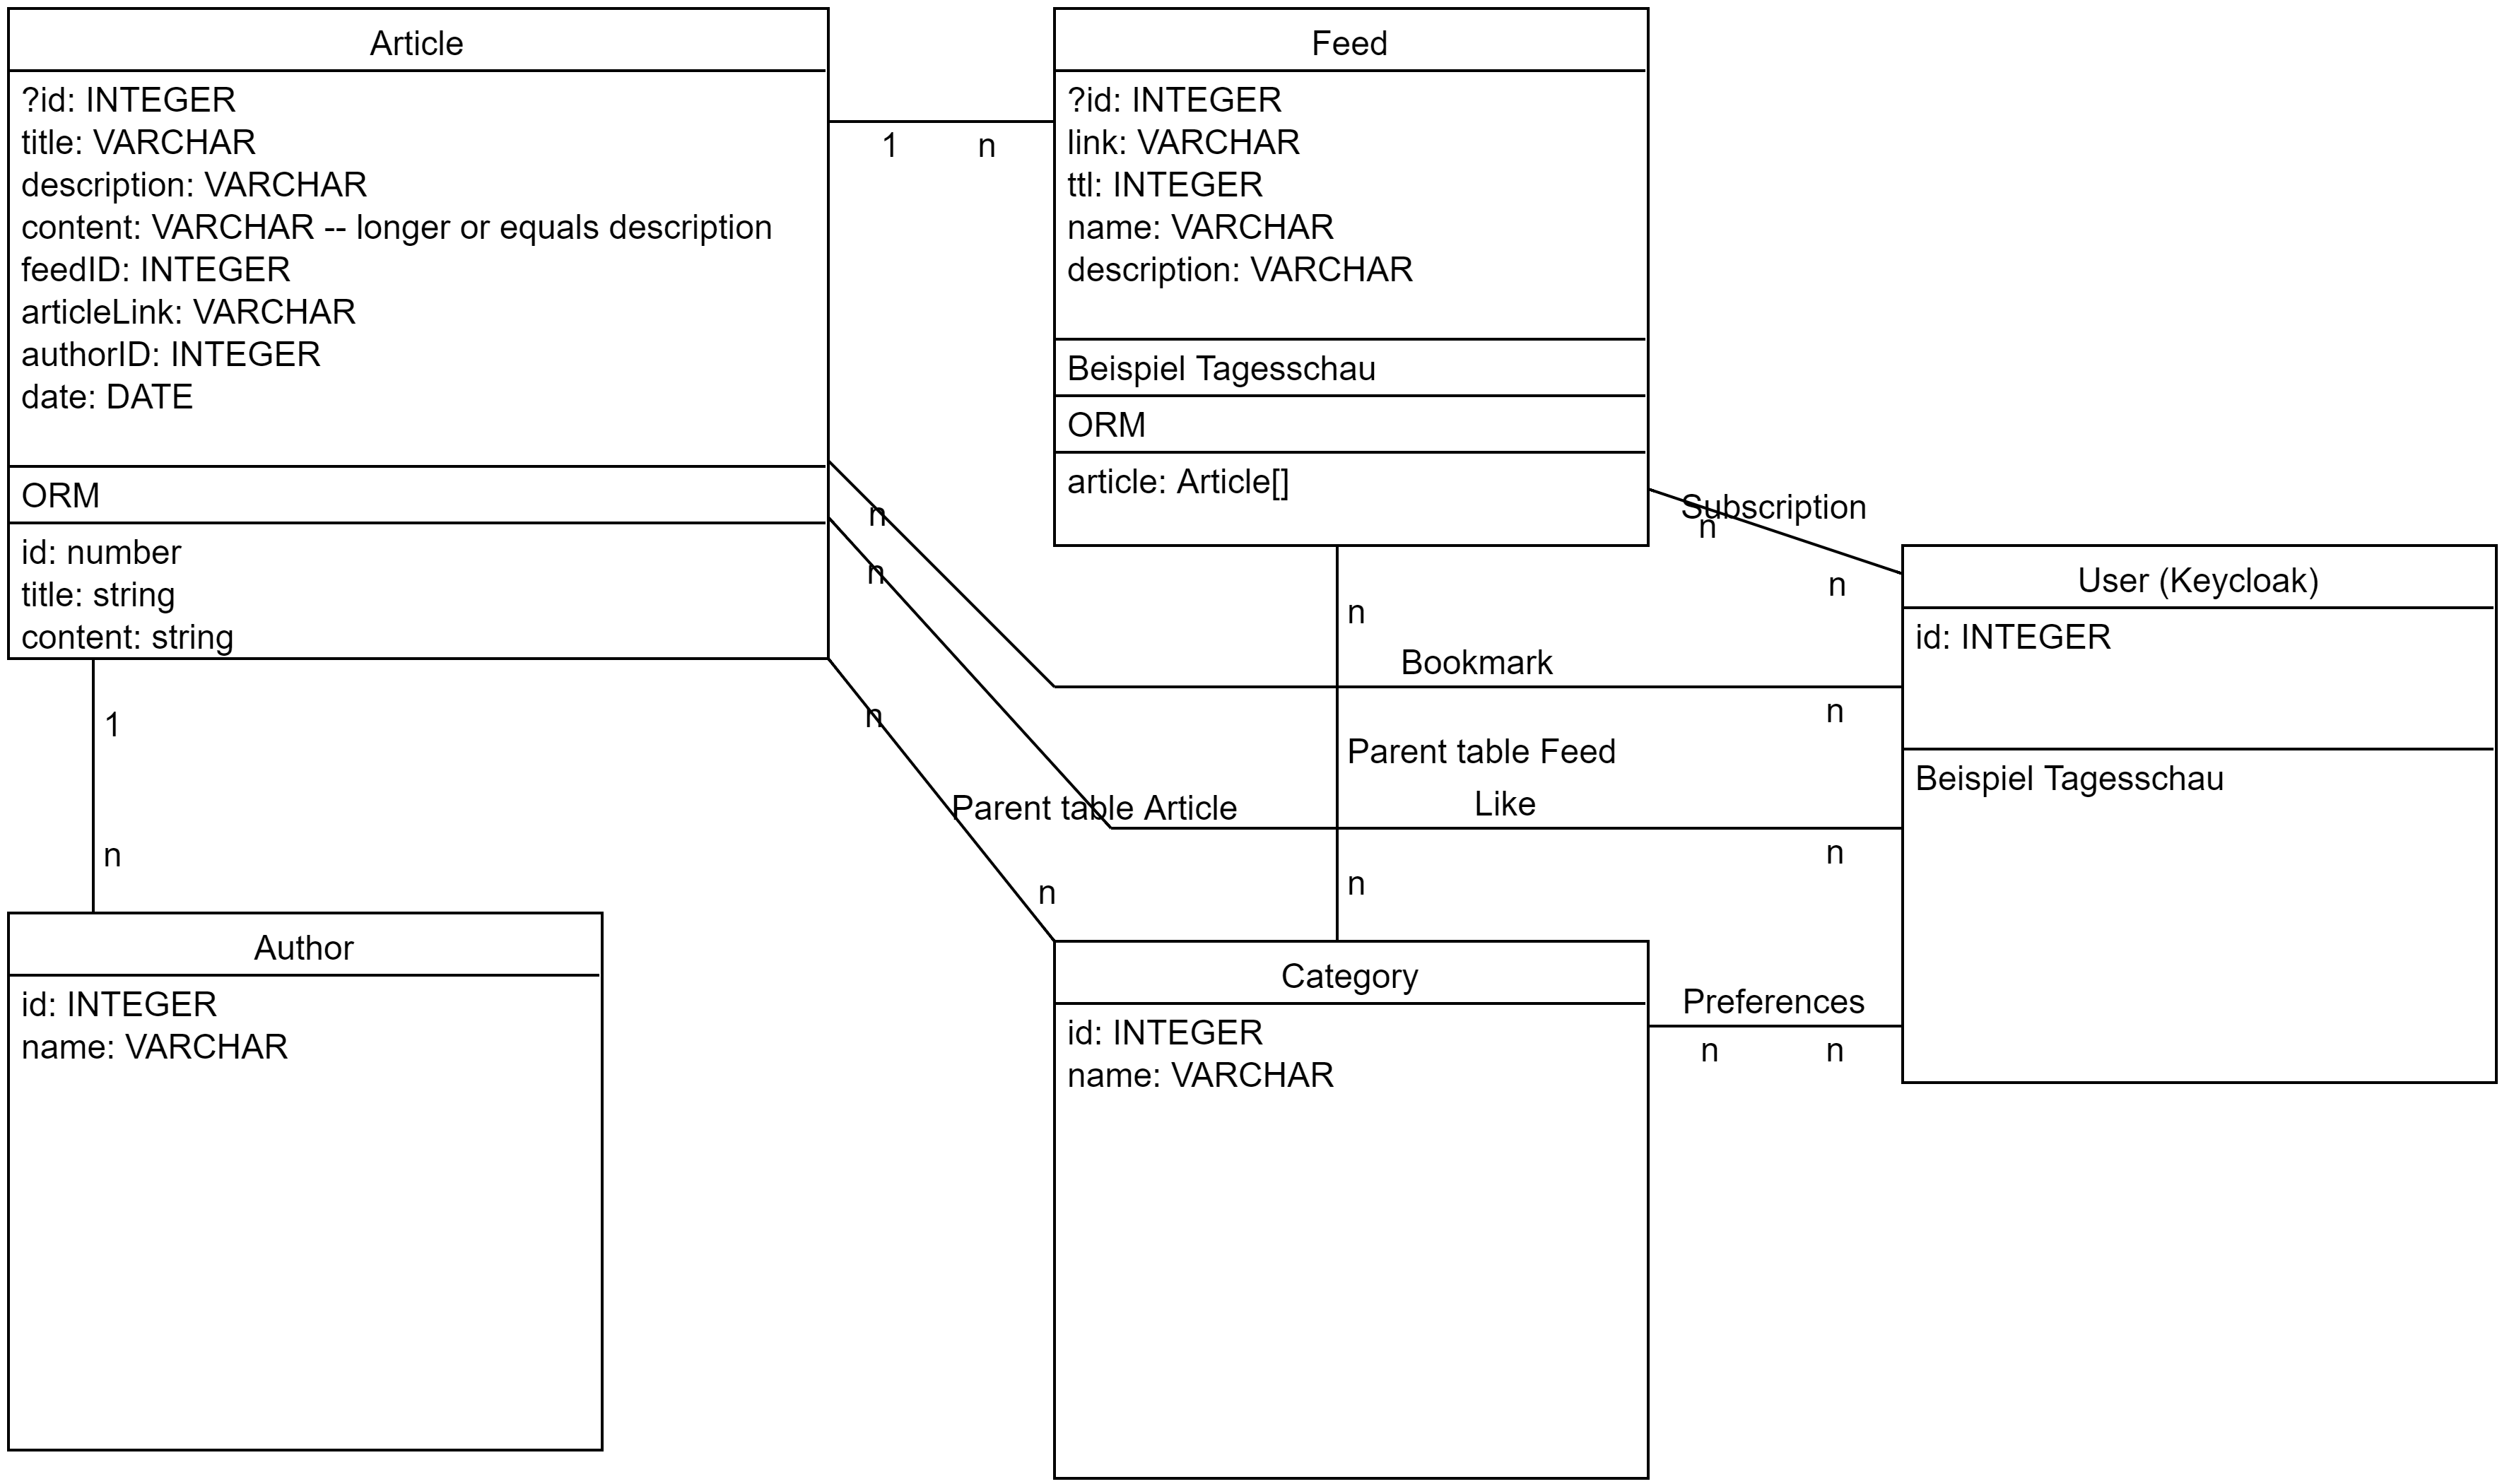
\includegraphics[width=\linewidth]{Database_Model.png}
    \caption{Datendefinition innerhalb der Datenbank}
    \label{fig:databaseORM}
\end{figure}
\end{quotation}
Bearbeitet von Jonas Eppard und Tim Horlacher.

\subsubsection{SKIOS-74 Extend workflow to include wontfix}
Das Ticket \enquote{SKIOS-74 Extend workflow to include wontfix} hatte folgende User Story:
\begin{quotation}
    As a team member, I would like a wontfix state to disregard tickets.
    Goal of this story is to modify the current issue workflow used by jira.
    Note: this might require admin rights (contact PO or Architect for this) \\
    \textbf{Acceptance Criteria}
    \begin{itemize}
        \item Wontfix status exists
        \item The status contains the done property (is striked out)
    \end{itemize}
\end{quotation}
Bearbeitet von Lukas Huida.
Reviewed von Amos Groß.

\subsubsection{SKIOS-85 Repeated Polling runs}
Das Ticket \enquote{SKIOS-85 Repeated Polling runs} hatte folgende User Story:
\begin{quotation}
    As a developer I would like the polling service to be run as a cron job. \\
    \textbf{Acceptance Criteria}
    \begin{itemize}
        \item Polling service is called in Intervalls.
        \item Pod is not running all the time.
    \end{itemize}
\end{quotation}
Bearbeitet von Lukas Huida.
Reviewed von Tim Horlacher.

\section{Sprint 3}

\subsection{Produktincrement}
\subsection{Charts}
\subsection{Probleme und Verbesserungen}


\subsection{Bearbeitete User Storys}
\subsubsection{SKIOS-116 Structure and table of contents for submission (\LaTeX)}
Das Ticket \enquote{SKIOS-116 Structure and table of contents for submission (\LaTeX)}
hatte folgende User Story:
\begin{quotation}
    As a team member, I would like to have a rough structure to orient myself while writing our submission documentation.\\
    For this story, please read the requirements and guidelines set out by Garidis and develop a rough idea on how to structure our \LaTeX project.\\
    \textbf{Acceptance Criteria}
    \begin{itemize}
        \item Table of contents is created (with \textbackslash{}section, \textbackslash{}subsection, etc.) in \LaTeX
        \item Structure reflects guidelines of Garidis
        \item Structure is explained in confluence page
        \item Existing \LaTeX~stories have a defined place where their pages will go
    \end{itemize}
\end{quotation}
Dies wurde folgendermaßen gelöst:
\begin{quotation}
    Es wurde die Struktur dieses \LaTeX-Dokuments angelegt. Hierbei musste nur das Inhaltsverzeichnis
    angelegt werden, da das \LaTeX-Template schon vorhanden war.
    Die Verwendung wurde in Confluence dokumentiert.
\end{quotation}
Bearbeitet von Jonas Eppard.

\subsubsection{SKIOS-73 Place new logo in git, jira, confluence, etc}
Das Ticket \enquote{SKIOS-73 Place new logo in git, Jira, confluence, etc} hatte folgende User Story:
\begin{quotation}
    As a Product Owner I want our logo to be placed in the git repository, Jira \& confluence. \\
    \textbf{Requirements}
    \begin{itemize}
        \item Add branding for Skiosa
        \item Possibly also change look of Jira (at the top) and make it use our colorscheme.  
    \end{itemize}   
    
    \textbf{Acceptance Criteria}
    \begin{itemize}
        \item Skiosa Brandig is present in Git and Jira.
    \end{itemize}
\end{quotation}
Bearbeitet von Lukas Huida.
Reviewed von Jonas Eppard.

\subsubsection{SKIOS-76 Automatic Reviewer Suggestions}
Das Ticket \enquote{SKIOS-76 Automatic Reviewer Suggestions} hatte folgende User Story:
\begin{quotation}
    As a developer I want to have a way to automatically suggest reviewers for a PR. \\
    \textbf{Acceptance Criteria}
    \begin{itemize}
        \item Added Codeowners to every repo.
    \end{itemize}
\end{quotation}
Bearbeitet von Lukas Huida.
Reviewed von Tim Horlacher.

\subsubsection{SKIOS-91 Checklist for PRs}
Das Ticket \enquote{SKIOS-91 Checklist for PRs} hatte folgende User Story:
\begin{quotation}
    As a developer, I would like to have a reminder to check off the checklist from our contributing guidelines. \\
    \textbf{Acceptance Criteria}
    \begin{itemize}
        \item Every PR contains comment or default text including the checklist.
    \end{itemize}
\end{quotation}
Bearbeitet von Lukas Huida.
Reviewed von Jonas Eppard.

\subsubsection{SKIOS-120 Deployment README}
Das Ticket \enquote{SKIOS-120 Deployment README} hatte folgende User Story:
\begin{quotation}
    As a developer, I would like a README in deployment so that I read up on information on how to use it. \\
\textbf{Acceptance Criteria}
\begin{itemize}
    \item README is created
    \item README includes:
    \begin{itemize}
        \item development guide (how to start application, use devcontainer)
        \item description of service
        \item requirements for service
        \item service lead
    \end{itemize}
\end{itemize}
\end{quotation}
Bearbeitet von Lukas Huida.
Reviewed von Amos Gross.

\subsubsection{SKIOS-138 Use Keycloak in GraphQL}
Das Ticket \enquote{SKIOS-138 Use Keycloak in GraphQL} hatte folgende User Story:
\begin{quotation}
    As a developer I want to secure some GraphQL resolver with our Keycloak. \\
    \textbf{Acceptance Criteria}
    \begin{itemize}
        \item Every resolver can be secured with Keycloak.
        \item An example resolver is created with Keycloak authentication.
    \end{itemize}
\end{quotation}
Bearbeitet von Lukas Huida.
Reviewed von Tim Horlacher.

\subsubsection{SKIOS-133 ORM Readme}
Das Ticket \enquote{SKIOS-133 ORM Readme} hatte folgende User Story:
\begin{quotation}
    As a developer, I would like a README for ORM so that I read up on information on how to use it. \\
\textbf{Acceptance Criteria}
\begin{itemize}
    \item README is created
    \item README includes:
    \begin{itemize}
        \item development guide (how to create tags and to embed it to package.json)
        \item description of what this module does
        \item code owners 
    \end{itemize}
\end{itemize}
\end{quotation}
Bearbeitet von Jonas Eppard.
Reviewed von Lukas Huida.
